\cbstart
\citeauthor{Heer2007} describe a tool called DynaVis which makes use of animated transitions between different visualisations. Users often switch the type of a visualisation in order to answer different questions concerning underlying data. However, doing this transition in a static way leads to information loss of the former visualisation. However, animating the transition of the current visualisation to the upcoming one could result in better comprehensibility of the upcoming visualisation. The cruical point of an animated transition is to keep the users oriented during the transition. The best case of an animated transition would be that users are able to accurately identify elments across disparate visualisations and understand the connections between them.

\citeauthor{Heer2007} investigate the design of animated transitions between statistical data graphics. Furthermore, they propose design guidelines for animated transitions which are discussed below. The primary contribution of \citeauthor{Heer2007} is two conducted user studies to assess the efficiency of animated transitions \iacite{Heer2007}.

The following design principles can be categorized into two sections: congruence and apprehension. All principles are taken from \citeauthor{Heer2007} and each one of them is listed and shortly discussed below \iacite{Heer2007}.
\begin{itemize}
\item \textbf{Congruence}
\begin{description}
\item[Maintain valid data graphics during transitions.] This design principle suggests that the interpolation states between two visualisations remain valid data graphics in order to minimize unwarranted attributions to the data.
\item[Use consistent semantic-syntactic mappings.] This principle recommends to use similar transitions for a single purpose throughout the visualisation tool. This ensures consistency across all available visualisation types.
\item[Respect semantic correspondence.] If a mark represents specific data points, it should not be reused to depict different data points in a transition.
\item[Avoid ambiguity] because it increases the risk of misinterpretation.
\end{description}

\item \textbf{Apprehension}
\begin{description}
\item[Group similar transitions.] Objects undergoing similar visual changes at the same time support comprehensibility of users due do perceptual grouping.
\item[Minimize occlusion.] Tracking occluding objects during a transitoin is unreasonable and also harming perception.
\item[Maximizing predictability] of a transition reduces cognitive load and improved tracking abilities.
\item[Use simple transitions] because complex transitions with unpredictable transitions would increase cognitive load.
\item[Use staging for complex transitions.] This allows for breaking down complex transitions into simple ones. Staging multiple simple transitions decreases cognitive load increases observability.
\item[Make transitions as long as needed, but no longer.] Slow transitions can result in longer task times and diminished engagement. However, they should still be long enough for accuracte change tracking.
\end{description}

\end{itemize}

DynaVis is shown in Figure \ref{fig:dynavis} on page \pageref{fig:dynavis}. It features two different types of animated transitions from a scatter plot to a bar chart. The top path directly interpolates between the starting and ending visualisation, whereas the bottom path makes use of staging. The points in the scatter plot move to their corresponding x-coordinate and the axis is updated. Afterwards, the points are morphed into bars resulting in the desired visualisation.
\cbend

\begin{figure}[!htb]
\centering
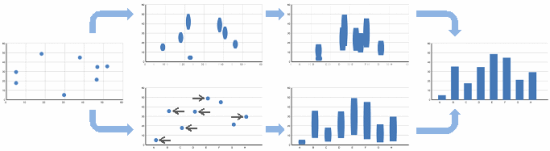
\includegraphics[width=0.8\textwidth, keepaspectratio]{images/methods/related/dynavis.png}
\caption[
    DynaVis \iacite{Heer2007}.
]{DynaVis}
\label{fig:dynavis}
\end{figure}

\cbstart
The herein before mentioned conducted user studies concerning the effectiveness of DynaVis showed, that animated transitions support the user's perception and increases the readability of the visualisation. Furthermore, the studies showed that staged animations are preferred compared to direct interpolations.

All in all, using staged animations with considering the mentioned design principles could also work for geo-spatial visualisations. Thus, it could support the understandability and readability of different types of geo-spatial visualisations.
\cbend